% Options for packages loaded elsewhere
\PassOptionsToPackage{unicode}{hyperref}
\PassOptionsToPackage{hyphens}{url}
%
\documentclass[
  ignorenonframetext,
]{beamer}
\usepackage{pgfpages}
\setbeamertemplate{caption}[numbered]
\setbeamertemplate{caption label separator}{: }
\setbeamercolor{caption name}{fg=normal text.fg}
\beamertemplatenavigationsymbolshorizontal
% Prevent slide breaks in the middle of a paragraph
\widowpenalties 1 10000
\raggedbottom
\setbeamertemplate{part page}{
  \centering
  \begin{beamercolorbox}[sep=16pt,center]{part title}
    \usebeamerfont{part title}\insertpart\par
  \end{beamercolorbox}
}
\setbeamertemplate{section page}{
  \centering
  \begin{beamercolorbox}[sep=12pt,center]{part title}
    \usebeamerfont{section title}\insertsection\par
  \end{beamercolorbox}
}
\setbeamertemplate{subsection page}{
  \centering
  \begin{beamercolorbox}[sep=8pt,center]{part title}
    \usebeamerfont{subsection title}\insertsubsection\par
  \end{beamercolorbox}
}
\AtBeginPart{
  \frame{\partpage}
}
\AtBeginSection{
  \ifbibliography
  \else
    \frame{\sectionpage}
  \fi
}
\AtBeginSubsection{
  \frame{\subsectionpage}
}

\usepackage{amsmath,amssymb}
\usepackage{lmodern}
\usepackage{iftex}
\ifPDFTeX
  \usepackage[T1]{fontenc}
  \usepackage[utf8]{inputenc}
  \usepackage{textcomp} % provide euro and other symbols
\else % if luatex or xetex
  \usepackage{unicode-math}
  \defaultfontfeatures{Scale=MatchLowercase}
  \defaultfontfeatures[\rmfamily]{Ligatures=TeX,Scale=1}
\fi
\usetheme[]{Antibes}
\usecolortheme{default}
% Use upquote if available, for straight quotes in verbatim environments
\IfFileExists{upquote.sty}{\usepackage{upquote}}{}
\IfFileExists{microtype.sty}{% use microtype if available
  \usepackage[]{microtype}
  \UseMicrotypeSet[protrusion]{basicmath} % disable protrusion for tt fonts
}{}
\makeatletter
\@ifundefined{KOMAClassName}{% if non-KOMA class
  \IfFileExists{parskip.sty}{%
    \usepackage{parskip}
  }{% else
    \setlength{\parindent}{0pt}
    \setlength{\parskip}{6pt plus 2pt minus 1pt}}
}{% if KOMA class
  \KOMAoptions{parskip=half}}
\makeatother
\usepackage{xcolor}
\newif\ifbibliography
\setlength{\emergencystretch}{3em} % prevent overfull lines
\setcounter{secnumdepth}{-\maxdimen} % remove section numbering

\usepackage{color}
\usepackage{fancyvrb}
\newcommand{\VerbBar}{|}
\newcommand{\VERB}{\Verb[commandchars=\\\{\}]}
\DefineVerbatimEnvironment{Highlighting}{Verbatim}{commandchars=\\\{\}}
% Add ',fontsize=\small' for more characters per line
\usepackage{framed}
\definecolor{shadecolor}{RGB}{241,243,245}
\newenvironment{Shaded}{\begin{snugshade}}{\end{snugshade}}
\newcommand{\AlertTok}[1]{\textcolor[rgb]{0.68,0.00,0.00}{#1}}
\newcommand{\AnnotationTok}[1]{\textcolor[rgb]{0.37,0.37,0.37}{#1}}
\newcommand{\AttributeTok}[1]{\textcolor[rgb]{0.40,0.45,0.13}{#1}}
\newcommand{\BaseNTok}[1]{\textcolor[rgb]{0.68,0.00,0.00}{#1}}
\newcommand{\BuiltInTok}[1]{\textcolor[rgb]{0.00,0.23,0.31}{#1}}
\newcommand{\CharTok}[1]{\textcolor[rgb]{0.13,0.47,0.30}{#1}}
\newcommand{\CommentTok}[1]{\textcolor[rgb]{0.37,0.37,0.37}{#1}}
\newcommand{\CommentVarTok}[1]{\textcolor[rgb]{0.37,0.37,0.37}{\textit{#1}}}
\newcommand{\ConstantTok}[1]{\textcolor[rgb]{0.56,0.35,0.01}{#1}}
\newcommand{\ControlFlowTok}[1]{\textcolor[rgb]{0.00,0.23,0.31}{#1}}
\newcommand{\DataTypeTok}[1]{\textcolor[rgb]{0.68,0.00,0.00}{#1}}
\newcommand{\DecValTok}[1]{\textcolor[rgb]{0.68,0.00,0.00}{#1}}
\newcommand{\DocumentationTok}[1]{\textcolor[rgb]{0.37,0.37,0.37}{\textit{#1}}}
\newcommand{\ErrorTok}[1]{\textcolor[rgb]{0.68,0.00,0.00}{#1}}
\newcommand{\ExtensionTok}[1]{\textcolor[rgb]{0.00,0.23,0.31}{#1}}
\newcommand{\FloatTok}[1]{\textcolor[rgb]{0.68,0.00,0.00}{#1}}
\newcommand{\FunctionTok}[1]{\textcolor[rgb]{0.28,0.35,0.67}{#1}}
\newcommand{\ImportTok}[1]{\textcolor[rgb]{0.00,0.46,0.62}{#1}}
\newcommand{\InformationTok}[1]{\textcolor[rgb]{0.37,0.37,0.37}{#1}}
\newcommand{\KeywordTok}[1]{\textcolor[rgb]{0.00,0.23,0.31}{#1}}
\newcommand{\NormalTok}[1]{\textcolor[rgb]{0.00,0.23,0.31}{#1}}
\newcommand{\OperatorTok}[1]{\textcolor[rgb]{0.37,0.37,0.37}{#1}}
\newcommand{\OtherTok}[1]{\textcolor[rgb]{0.00,0.23,0.31}{#1}}
\newcommand{\PreprocessorTok}[1]{\textcolor[rgb]{0.68,0.00,0.00}{#1}}
\newcommand{\RegionMarkerTok}[1]{\textcolor[rgb]{0.00,0.23,0.31}{#1}}
\newcommand{\SpecialCharTok}[1]{\textcolor[rgb]{0.37,0.37,0.37}{#1}}
\newcommand{\SpecialStringTok}[1]{\textcolor[rgb]{0.13,0.47,0.30}{#1}}
\newcommand{\StringTok}[1]{\textcolor[rgb]{0.13,0.47,0.30}{#1}}
\newcommand{\VariableTok}[1]{\textcolor[rgb]{0.07,0.07,0.07}{#1}}
\newcommand{\VerbatimStringTok}[1]{\textcolor[rgb]{0.13,0.47,0.30}{#1}}
\newcommand{\WarningTok}[1]{\textcolor[rgb]{0.37,0.37,0.37}{\textit{#1}}}

\providecommand{\tightlist}{%
  \setlength{\itemsep}{0pt}\setlength{\parskip}{0pt}}\usepackage{longtable,booktabs,array}
\usepackage{calc} % for calculating minipage widths
\usepackage{caption}
% Make caption package work with longtable
\makeatletter
\def\fnum@table{\tablename~\thetable}
\makeatother
\usepackage{graphicx}
\makeatletter
\def\maxwidth{\ifdim\Gin@nat@width>\linewidth\linewidth\else\Gin@nat@width\fi}
\def\maxheight{\ifdim\Gin@nat@height>\textheight\textheight\else\Gin@nat@height\fi}
\makeatother
% Scale images if necessary, so that they will not overflow the page
% margins by default, and it is still possible to overwrite the defaults
% using explicit options in \includegraphics[width, height, ...]{}
\setkeys{Gin}{width=\maxwidth,height=\maxheight,keepaspectratio}
% Set default figure placement to htbp
\makeatletter
\def\fps@figure{htbp}
\makeatother

\logo{
\includegraphics[width=2cm]{figures/udem.png}}
\usepackage{copyrightbox}
\usepackage{dirtree}
\usepackage{forest}
\makeatletter
\makeatother
\makeatletter
\makeatother
\makeatletter
\@ifpackageloaded{caption}{}{\usepackage{caption}}
\AtBeginDocument{%
\ifdefined\contentsname
  \renewcommand*\contentsname{Table of contents}
\else
  \newcommand\contentsname{Table of contents}
\fi
\ifdefined\listfigurename
  \renewcommand*\listfigurename{List of Figures}
\else
  \newcommand\listfigurename{List of Figures}
\fi
\ifdefined\listtablename
  \renewcommand*\listtablename{List of Tables}
\else
  \newcommand\listtablename{List of Tables}
\fi
\ifdefined\figurename
  \renewcommand*\figurename{Figure}
\else
  \newcommand\figurename{Figure}
\fi
\ifdefined\tablename
  \renewcommand*\tablename{Table}
\else
  \newcommand\tablename{Table}
\fi
}
\@ifpackageloaded{float}{}{\usepackage{float}}
\floatstyle{ruled}
\@ifundefined{c@chapter}{\newfloat{codelisting}{h}{lop}}{\newfloat{codelisting}{h}{lop}[chapter]}
\floatname{codelisting}{Listing}
\newcommand*\listoflistings{\listof{codelisting}{List of Listings}}
\makeatother
\makeatletter
\@ifpackageloaded{caption}{}{\usepackage{caption}}
\@ifpackageloaded{subcaption}{}{\usepackage{subcaption}}
\makeatother
\makeatletter
\@ifpackageloaded{tcolorbox}{}{\usepackage[many]{tcolorbox}}
\makeatother
\makeatletter
\@ifundefined{shadecolor}{\definecolor{shadecolor}{rgb}{.97, .97, .97}}
\makeatother
\makeatletter
\makeatother
\ifLuaTeX
  \usepackage{selnolig}  % disable illegal ligatures
\fi
\IfFileExists{bookmark.sty}{\usepackage{bookmark}}{\usepackage{hyperref}}
\IfFileExists{xurl.sty}{\usepackage{xurl}}{} % add URL line breaks if available
\urlstyle{same} % disable monospaced font for URLs
\hypersetup{
  pdftitle={Reproducible papers in the life sciences using R},
  hidelinks,
  pdfcreator={LaTeX via pandoc}}

\title{Reproducible papers in the life sciences using R}
\author{Ariel Mundo Ortiz}
\date{CANSSI Statistical Software Conference\\
November 10, 2022}
\institute{Université de Montréal\\
\strut \\

\includegraphics[width=0.6cm]{figures/Twitter.png} @amundortiz\\
\strut \\

\includegraphics[width=0.6cm]{figures/Mastodon.png} @aimundo}

\begin{document}
\frame{\titlepage}
\ifdefined\Shaded\renewenvironment{Shaded}{\begin{tcolorbox}[sharp corners, frame hidden, interior hidden, borderline west={3pt}{0pt}{shadecolor}, boxrule=0pt, breakable, enhanced]}{\end{tcolorbox}}\fi

\begin{frame}[fragile]{Introduction}
\protect\hypertarget{introduction}{}
\begin{itemize}[<+->]
\item
  \texttt{RMarkdown} is a powerful tool to create reproducible papers
\item
  However, R is rarely used in the life sciences as a default method to
  create papers
\item
  \color{red}{Why?}
\end{itemize}
\end{frame}

\begin{frame}{Reasons}
\protect\hypertarget{reasons}{}
\begin{itemize}[<+->]
\tightlist
\item
  ``R is just for Stats''
\item
  ``There is a learning curve''
\item
  \textbf{``I can't create figures for publication''}
\end{itemize}
\end{frame}

\begin{frame}{The Problem}
\protect\hypertarget{the-problem}{}
\begin{itemize}[<+->]
\tightlist
\item
  Papers in the life sciences usually require figures where the
  following are combined:

  \begin{itemize}[<+->]
  \tightlist
  \item
    Images from cells/tissues
  \item
    Figures that summarize data
  \item
    Figures that present statistical analyses (with ``p-values'')
  \end{itemize}
\end{itemize}
\end{frame}

\begin{frame}{The Problem}
\protect\hypertarget{the-problem-1}{}
\begin{figure}
\centering
\caption{A typical figure}
\copyrightbox[b]{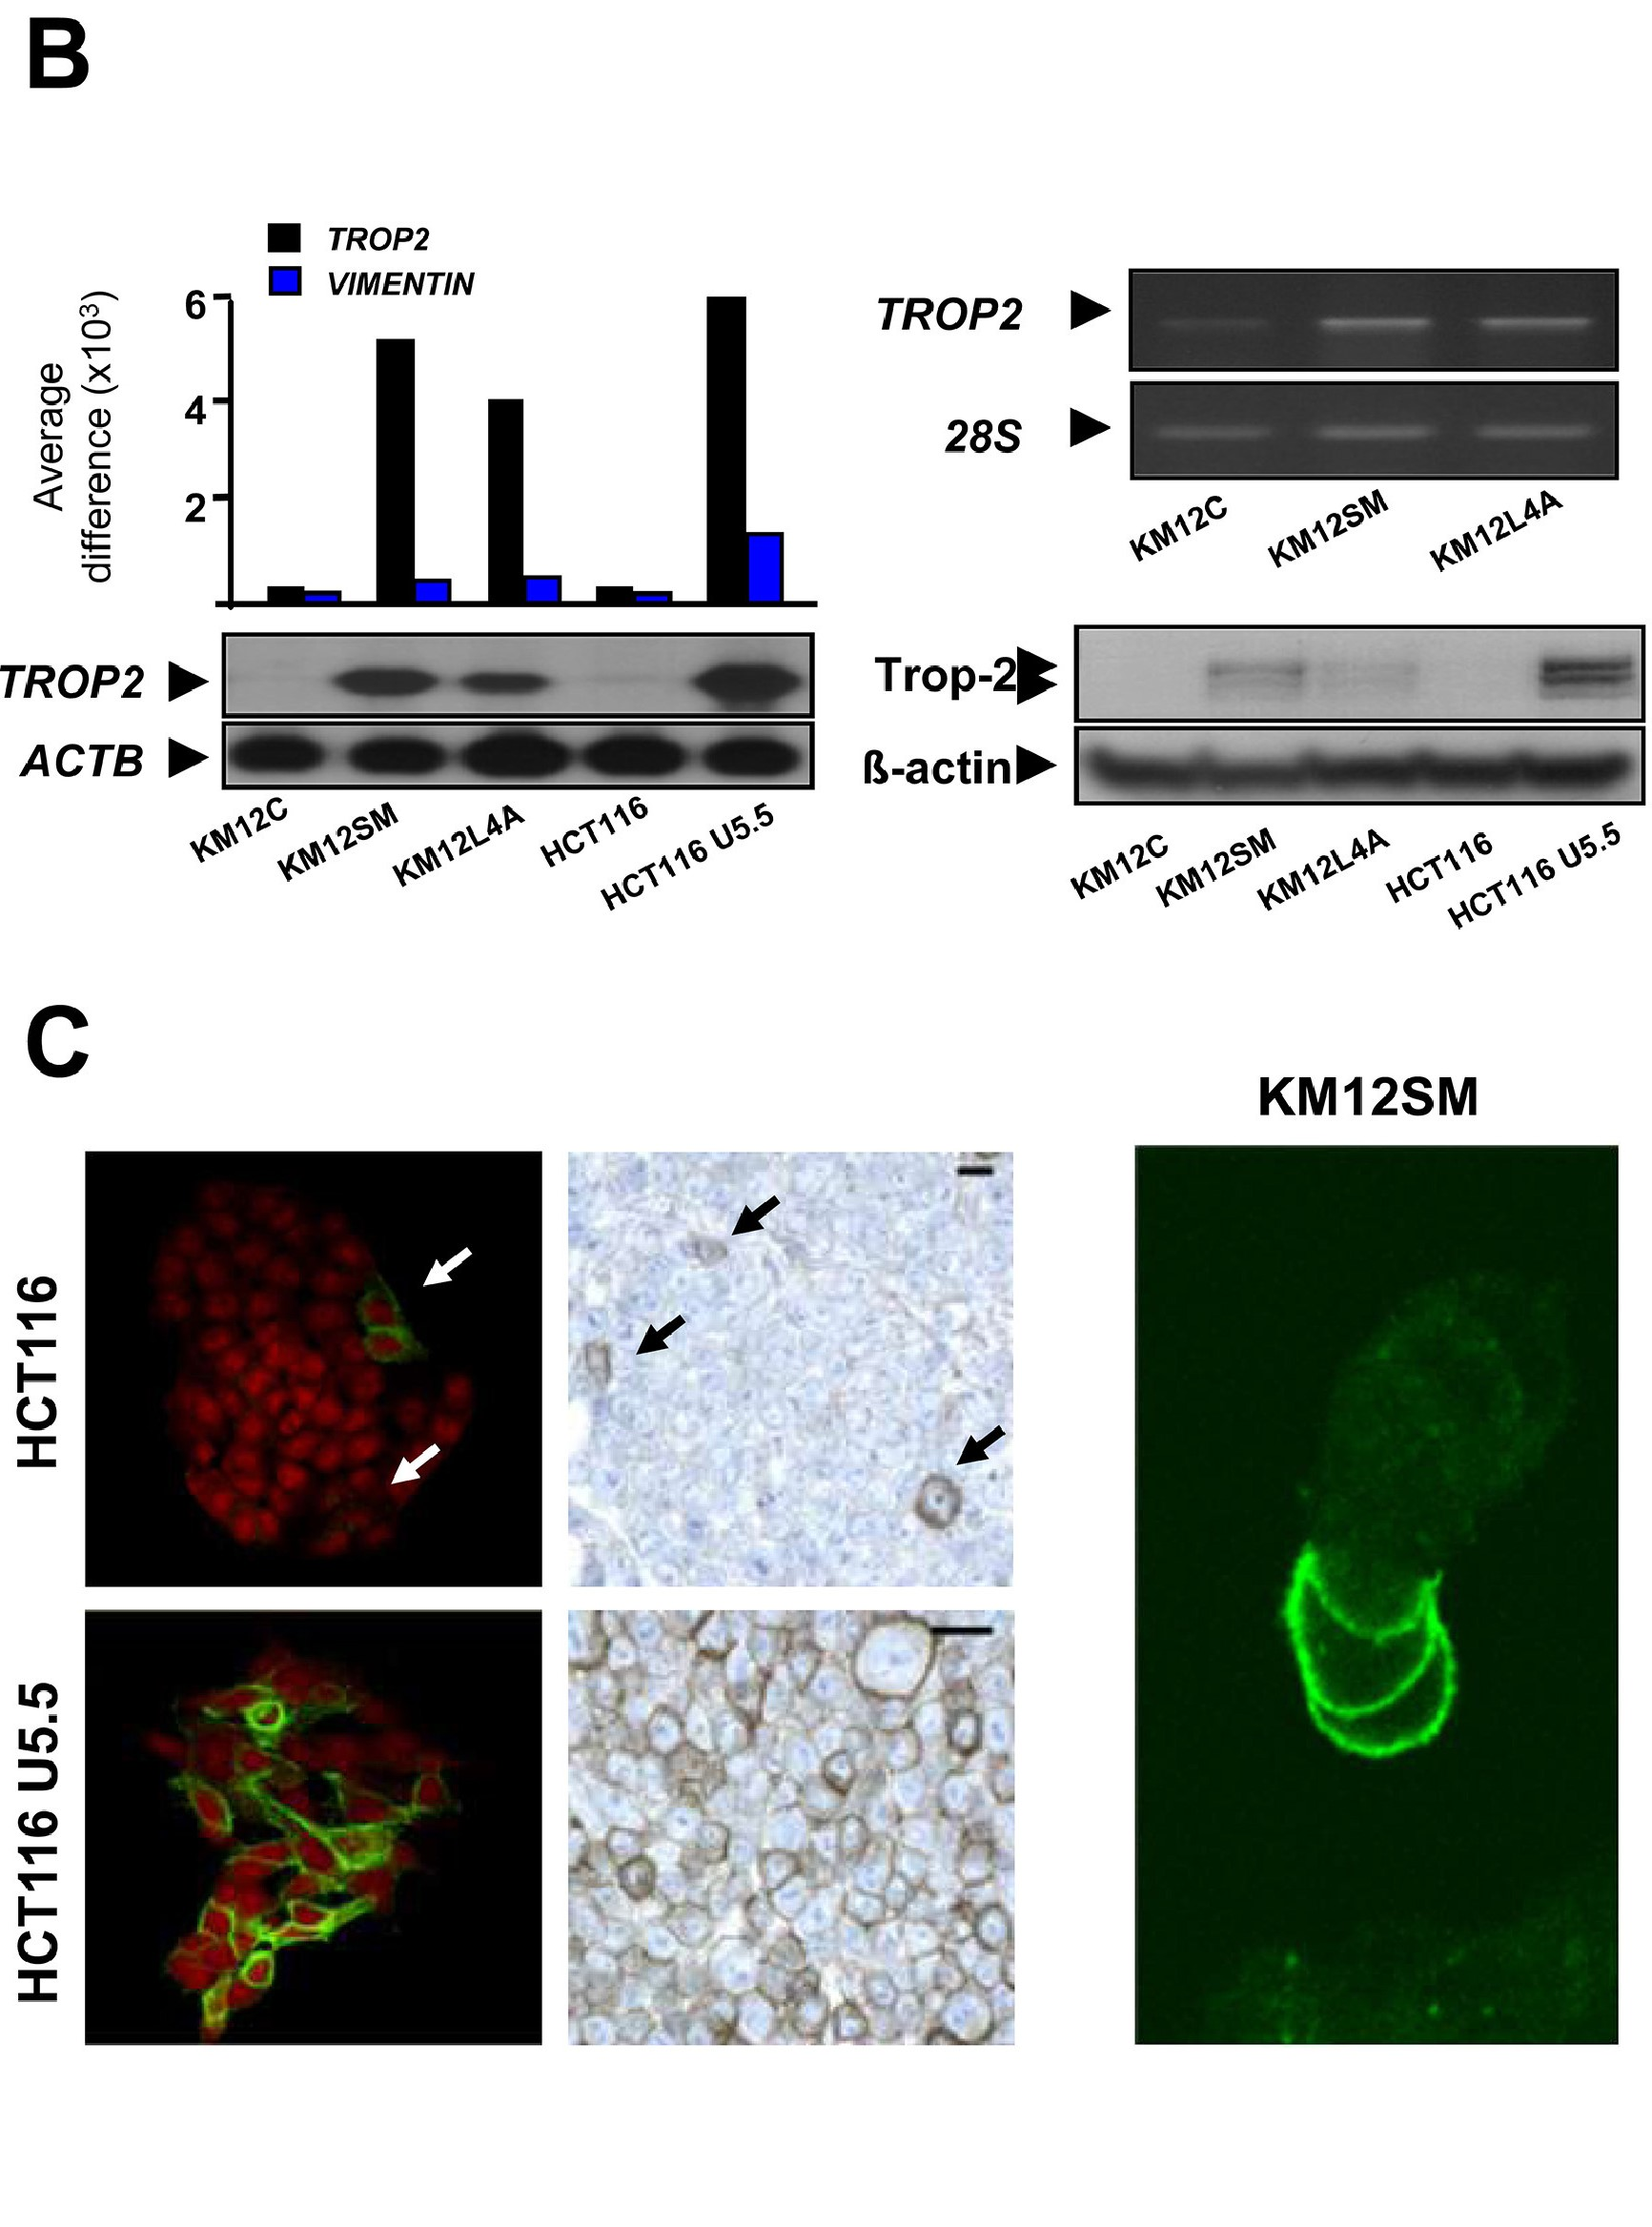
\includegraphics[width=2.5cm]{figures/figure.jpg}}
                {\tiny{Guerra et al.} \textit{Neoplasia} \textbf{2021}}
    \end{figure}

\begin{itemize}[<+->]
\item
  \color{red}{Can figures like this be created using `RMarkdown`?}
\end{itemize}
\end{frame}

\begin{frame}{The Solution}
\protect\hypertarget{the-solution}{}
\begin{itemize}[<+->]
\item
  Yes, we can create figures like this using R!
\item
  We will need to use a combination of packages to achieve this
\end{itemize}

\begin{figure}
\centering
\caption{The packages}
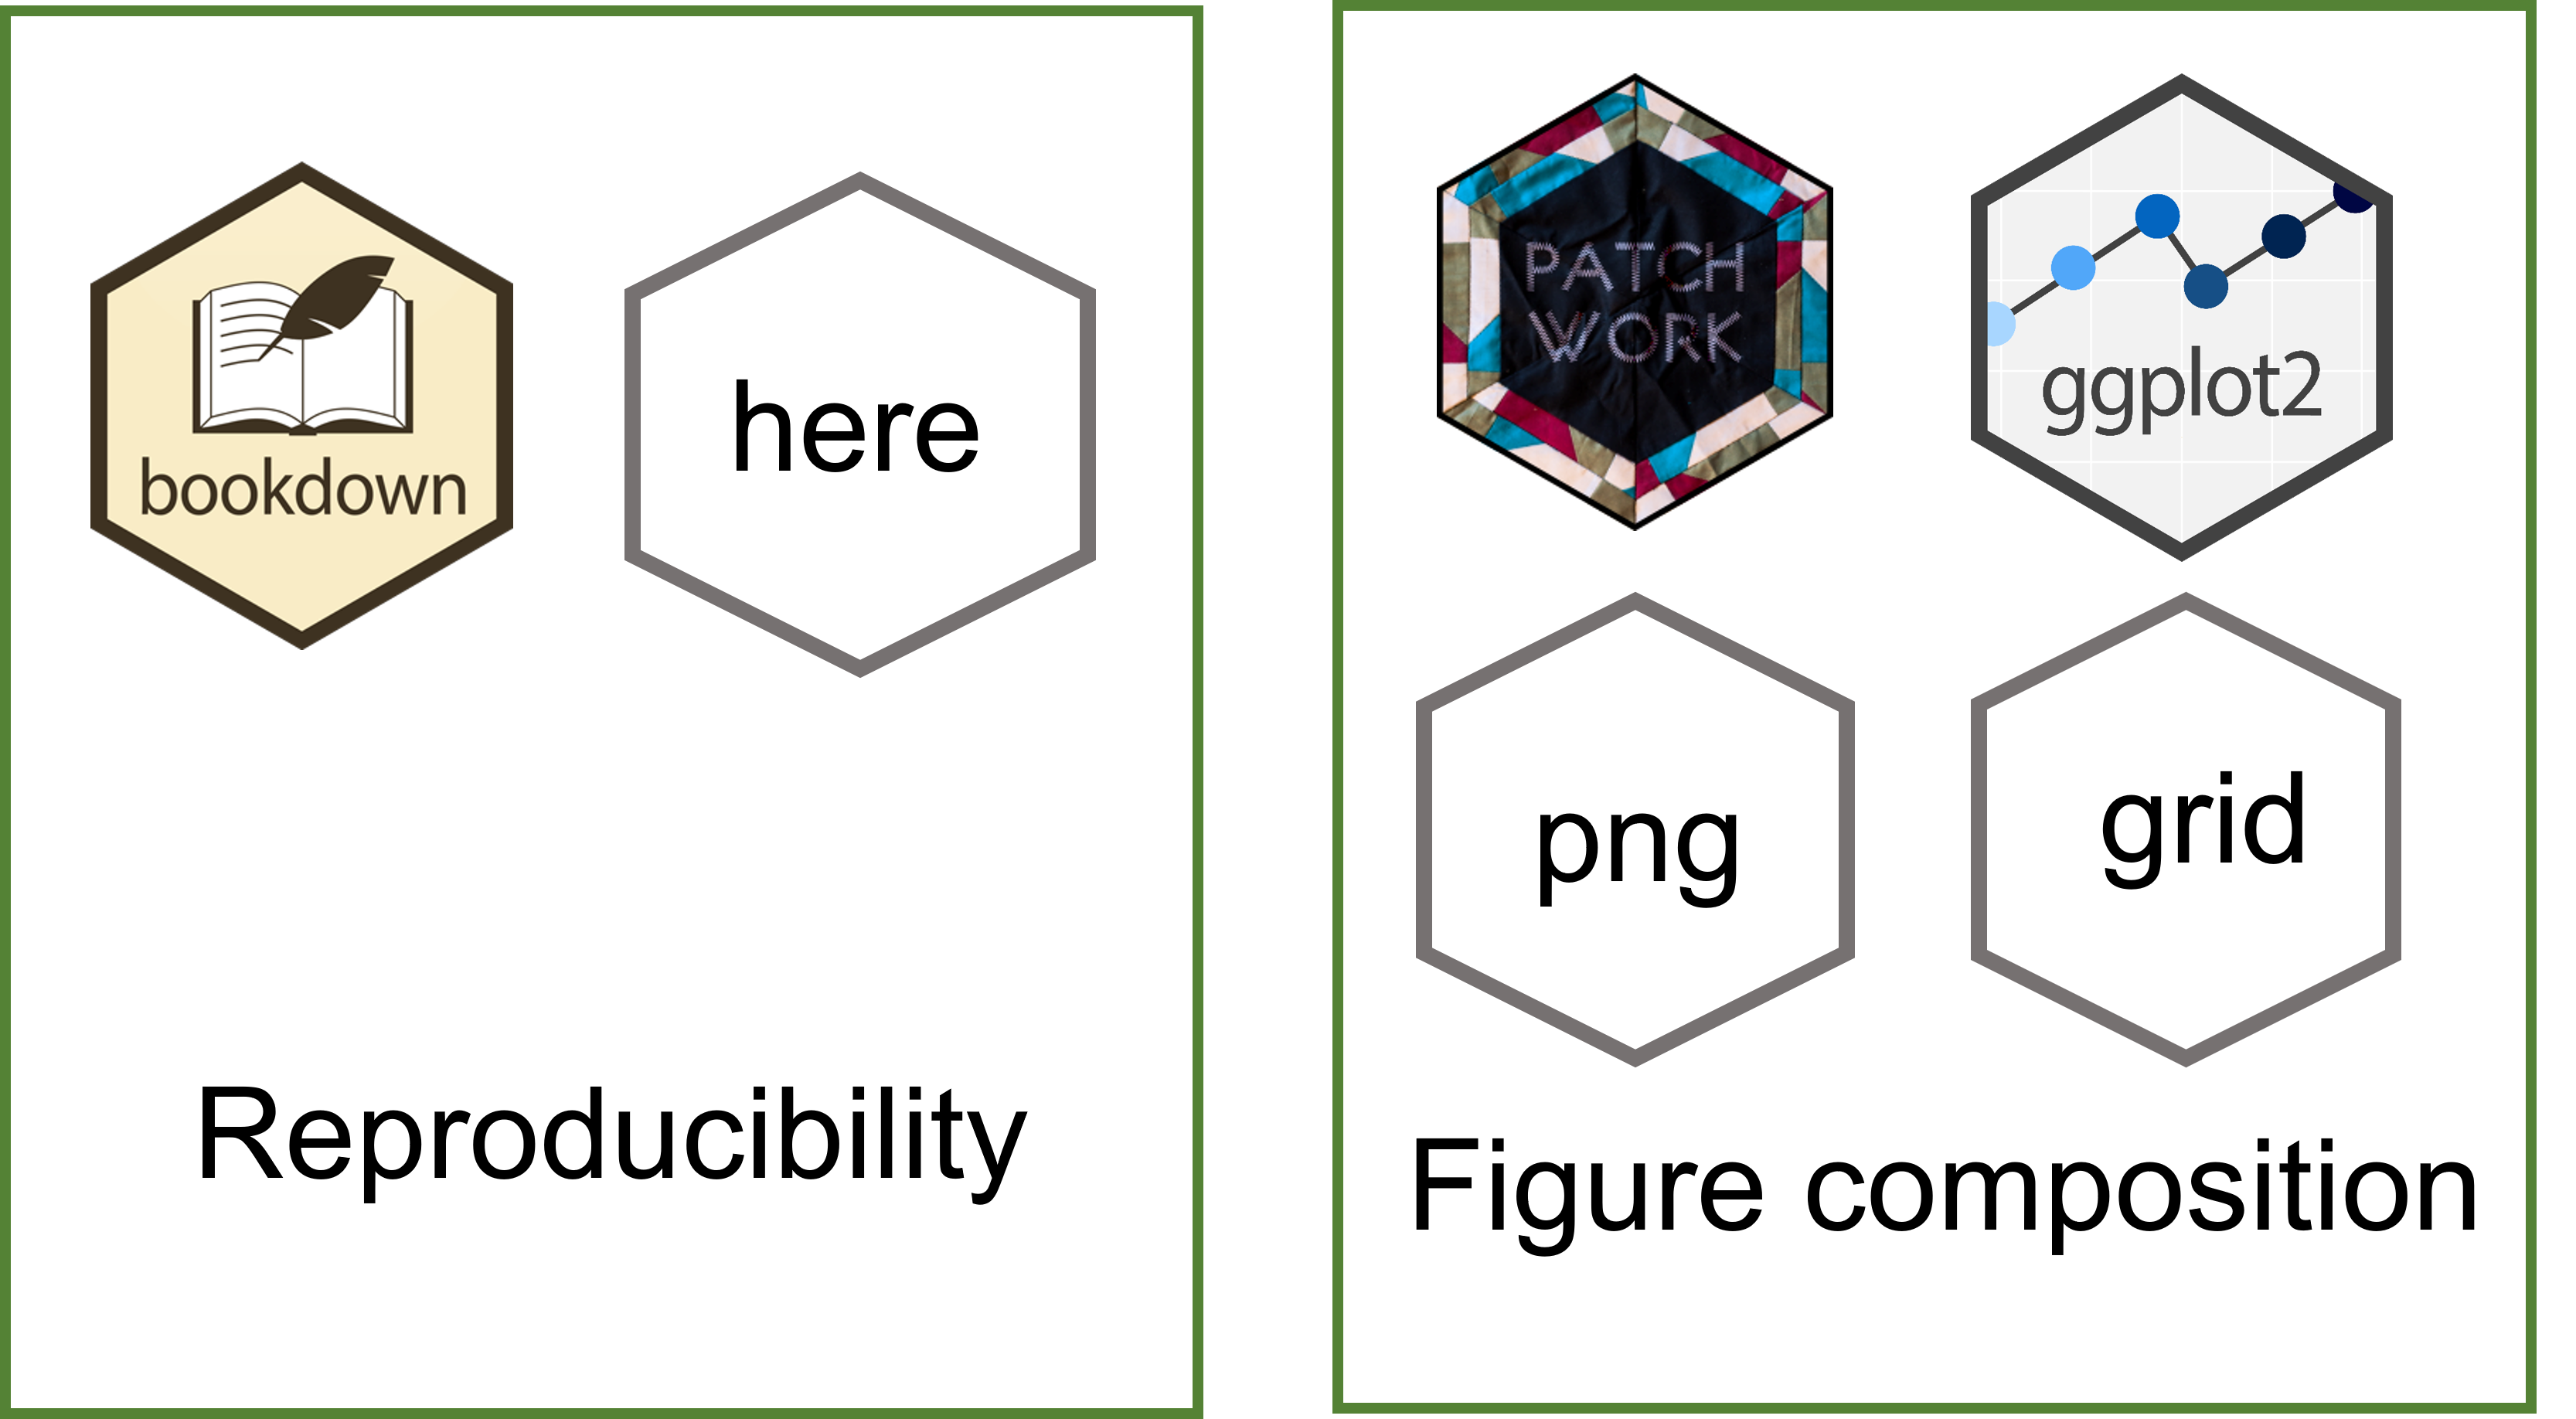
\includegraphics[width=6cm]{figures/R_packages.png}
\end{figure}
\end{frame}

\begin{frame}[fragile]{The Solution}
\protect\hypertarget{the-solution-1}{}
\begin{itemize}[<+->]
\tightlist
\item
  \textcolor{green}{{bookdown}} allows to create a reproducible paper:

  \begin{itemize}[<+->]
  \tightlist
  \item
    Each section of the paper: (Materials and Methods, Results, etc.) is
    in a separate \texttt{Rmd} file
  \item
    More details can be found in \url{https://bookdown.org/}
  \end{itemize}
\item
  \textcolor{green}{{here}} allows to easily call scripts within the
  document (we will look at this later)
\end{itemize}
\end{frame}

\begin{frame}[fragile]{The Solution}
\protect\hypertarget{the-solution-2}{}
\begin{itemize}[<+->]
\tightlist
\item
  Let's think about a typical scenario, where you:

  \begin{itemize}[<+->]
  \item
    Have written your paper sections (Methods, Results, etc) each
    section is in a \texttt{Rmd} file
  \item
    Have some images
  \item
    Have some data that needs to be analyzed
  \item
    Want to create a composite figure of images/data analysis
  \item
    \textbf{For the sake of time, I will focus on the image
    composition/data analysis part}
  \end{itemize}
\end{itemize}
\end{frame}

\begin{frame}{Project Organization}
\protect\hypertarget{project-organization}{}
\begin{itemize}[<+->]
\tightlist
\item
  How to organize the files:
\end{itemize}

\pause

\footnotesize
\centering
\begin{forest}
        for tree={
            font=\ttfamily,
            text width=8cm,% added <<<<<<<<<<<<<<
            grow'=0,
            child anchor=west,
            parent anchor=south,
            anchor=west,
            calign=first,
            inner xsep=7pt,
            edge path={
                \noexpand\path [draw, \forestoption{edge}]
                (!u.south west) +(7.5pt,0) |- (.child anchor) 
                \forestoption{edge label};
            },
            before typesetting nodes={
                if n=1
                {insert before={[,phantom]}}
                {}
            },
            fit=band,
            before computing xy={l=15pt},
        }  
        [Project
        [Data
        [csv files
        ]
        ]
        [Code
        [R Script(s)
        ]
        ]
        [Figures
        [PNG (or other image files)
        ]
        ]
        [Manuscript
        [Rmd files (sections)
        ]
        ]
        ]
    \end{forest}

\normalsize
\end{frame}

\begin{frame}{A Handy Script: Images}
\protect\hypertarget{a-handy-script-images}{}
\begin{itemize}[<+->]
\tightlist
\item
  We can read the images (in PNG format), get the data, do the analysis
  and create the figure in a single script!

  \begin{itemize}[<+->]
  \tightlist
  \item
    Reading the images is achieved by \textcolor{green}{{grid}} and
    \textcolor{green}{{png}}
  \item
    \textcolor{green}{{ggplot2}} creates the plot of our analysis
  \item
    \textcolor{green}{{patchwork}} allows us to assemble everything
  \end{itemize}
\end{itemize}
\end{frame}

\begin{frame}[fragile]{A Handy Script: Images}
\protect\hypertarget{a-handy-script-images-1}{}
\begin{itemize}[<+->]
\tightlist
\item
  How do we read a PNG image?
\end{itemize}

\footnotesize

\begin{Shaded}
\begin{Highlighting}[]
\NormalTok{cells}\OtherTok{\textless{}{-}}\FunctionTok{rasterGrob}\NormalTok{(}\FunctionTok{readPNG}\NormalTok{(}\FunctionTok{here}\NormalTok{(}\StringTok{"figures"}\NormalTok{,}
                               \StringTok{"cells.png"}\NormalTok{),}
                          \AttributeTok{native=}\ConstantTok{TRUE}\NormalTok{))}
\end{Highlighting}
\end{Shaded}

\normalsize

\begin{itemize}[<+->]
\tightlist
\item
  We use \textcolor{green}{{here}} to call the PNG file located in the
  ``figures'' directory.
\item
  \texttt{rasterGrob} makes the image a ``graphical object'' (grob) that
  can be invoked later
\end{itemize}
\end{frame}

\begin{frame}[fragile]{A Handy Script: Data Analysis}
\protect\hypertarget{a-handy-script-data-analysis}{}
\footnotesize

\begin{Shaded}
\begin{Highlighting}[]
\CommentTok{\# for regression}

\NormalTok{formula}\OtherTok{\textless{}{-}}\NormalTok{y}\SpecialCharTok{\textasciitilde{}}\NormalTok{x}

\CommentTok{\# create a plot of the data and the regression}
\NormalTok{a1}\OtherTok{\textless{}{-}}\FunctionTok{ggplot}\NormalTok{(}\AttributeTok{data=}\NormalTok{data,}
           \FunctionTok{aes}\NormalTok{(}\AttributeTok{x=}\NormalTok{weight,}\AttributeTok{y=}\NormalTok{body\_fat,}\AttributeTok{fill=}\NormalTok{Group,}\AttributeTok{color=}\NormalTok{Group)}
\NormalTok{           )}\SpecialCharTok{+}
    \FunctionTok{geom\_point}\NormalTok{(}\AttributeTok{show.legend=}\ConstantTok{FALSE}\NormalTok{,}\AttributeTok{shape=}\DecValTok{21}\NormalTok{,}\AttributeTok{colour=}\StringTok{\textquotesingle{}black\textquotesingle{}}\NormalTok{,}\AttributeTok{size=}\DecValTok{5}\NormalTok{,}
               \AttributeTok{alpha=}\FloatTok{0.7}\NormalTok{)}\SpecialCharTok{+}
    \FunctionTok{geom\_smooth}\NormalTok{(}\AttributeTok{method=}\StringTok{"lm"}\NormalTok{,}\AttributeTok{formula=}\NormalTok{formula, }\AttributeTok{se=}\NormalTok{T)}\SpecialCharTok{+}
    \FunctionTok{stat\_poly\_eq}\NormalTok{(}\FunctionTok{use\_label}\NormalTok{(}\FunctionTok{c}\NormalTok{(}\StringTok{"R2"}\NormalTok{,}\StringTok{"p.value"}\NormalTok{)), }
                 \AttributeTok{formula =}\NormalTok{ formula, }\AttributeTok{size =} \DecValTok{3}\NormalTok{)}
\end{Highlighting}
\end{Shaded}

\normalsize

\begin{itemize}[<+->]
\tightlist
\item
  Try \textcolor{green}{{ggpmisc}}
\end{itemize}
\end{frame}

\begin{frame}[fragile]{A Handy Script: Layout}
\protect\hypertarget{a-handy-script-layout}{}
\begin{itemize}[<+->]
\tightlist
\item
  Provide a layout for the figure
  (\url{https://patchwork.data-imaginist.com/articles/guides/layout.html})
\end{itemize}

\pause

\footnotesize

\begin{Shaded}
\begin{Highlighting}[]
\NormalTok{                        layout}\OtherTok{\textless{}{-}}\StringTok{"}
\StringTok{                        AAAABBBB}
\StringTok{                        AAAABBBB}
\StringTok{                        AAAABBBB}
\StringTok{                        AAAABBBB}
\StringTok{                        CCCCDDDD}
\StringTok{                        CCCCDDDD}
\StringTok{                        CCCCEEEE}
\StringTok{                        CCCCEEEE}
\StringTok{                        "}
\end{Highlighting}
\end{Shaded}
\end{frame}

\begin{frame}[fragile]{A Handy Script: Assemble!}
\protect\hypertarget{a-handy-script-assemble}{}
\begin{itemize}[<+->]
\tightlist
\item
  Use \texttt{wrap\_elements} and \textcolor{green}{{patchwork}}
\end{itemize}

\footnotesize

\begin{Shaded}
\begin{Highlighting}[]
\NormalTok{                image\_a}\OtherTok{\textless{}{-}}\FunctionTok{wrap\_elements}\NormalTok{(}
                    \AttributeTok{panel=}\NormalTok{cells}
\NormalTok{                )}\SpecialCharTok{+}
                    \FunctionTok{wrap\_elements}\NormalTok{(}
                        \AttributeTok{panel=}\NormalTok{molecule}
\NormalTok{                    )}\SpecialCharTok{+}
                    \FunctionTok{wrap\_elements}\NormalTok{(}
                        \AttributeTok{panel=}\NormalTok{jellyfish}
\NormalTok{                    )}\SpecialCharTok{+}
                    \FunctionTok{ylab}\NormalTok{(}\StringTok{"jellyfish"}\NormalTok{)}\SpecialCharTok{+}
\NormalTok{                    a1}\SpecialCharTok{+}
\NormalTok{                    a2}\SpecialCharTok{+}
                    \FunctionTok{plot\_layout}\NormalTok{(}\AttributeTok{design=}\NormalTok{layout)}
\end{Highlighting}
\end{Shaded}

\normalsize

(\textbf{go to script})
\end{frame}

\begin{frame}{Conclusion}
\protect\hypertarget{conclusion}{}
\begin{itemize}[<+->]
\tightlist
\item
  We can use R to create reproducible papers and complex figures
\item
  There \textbf{is} a learning curve, but once you learn you won't go
  back to W**d!
\end{itemize}
\end{frame}

\begin{frame}{Acknowlegdments}
\protect\hypertarget{acknowlegdments}{}
\begin{columns}
\begin{column}{0.6\textwidth}
\footnotesize
- Nasri Lab (Université de Montréal) \\
- Centre de recherches mathématiques (CRM)\\
- Mathematics for Public Health (MfPH)

\end{column}
\begin{column}{0.4\textwidth}
\vspace{0.01em}
\centering
        
\includegraphics[width=2cm]{figures/logo.png}\\
        
\includegraphics[width=2cm]{figures/espum.jpg}\\
        
\includegraphics[width=2cm]{figures/crm.png}\\
         
\includegraphics[width=2cm]{figures/mfph.png}\\
         
\end{column}
\end{columns}
\end{frame}



\end{document}
